
\begin{slide}{Motivation of Soot Attributes}
\begin{itemize}
\item We often want to attach annotations to code
\begin{itemize}
\item to convey low-level analysis results, such as register allocation or
      array bounds check elimination to a VM
\item to convey analysis results to humans
\item to record profiling information
\end{itemize}
\item Soot provides a framework to support the embedding of custom, 
      user-defined attributes in class files
\end{itemize}
\end{slide}

\begin{slide}{Java class file attributes}
\begin{itemize}
\item Attributes of {\em class\_info}, {\em method\_info}, 
      {\em field\_info}, and {\em Code\_attribute} structures
\item In fact: Code is an attribute of a method
\item Standard attributes: SourceFile, ConstantValue, Exceptions,
      LineNumberTable, LocalVariableTable
\item VM is required to ignore attributes it does not recognize
\end{itemize}
\end{slide}

\begin{slide}{Attribute format}
The VM spec defines the format of attributes:
\small{
\begin{verbatim}
attribute_info {
  u2 attribute_name_index;
  u4 attribute_length;
  u1 info[attribute_length];
}
\end{verbatim}
}
\begin{itemize}
\item {\tt attribute\_name\_index}, the index of the attribute's name in the class files' {\em Constant Pool}
\item {\tt attribute\_length}, the length of the attribute's data
\item {\tt info}, an array of raw attribute data
\end{itemize}
\end{slide}

\begin{slide}{Attributes and Soot (overview)}
\vspace*{-5mm}
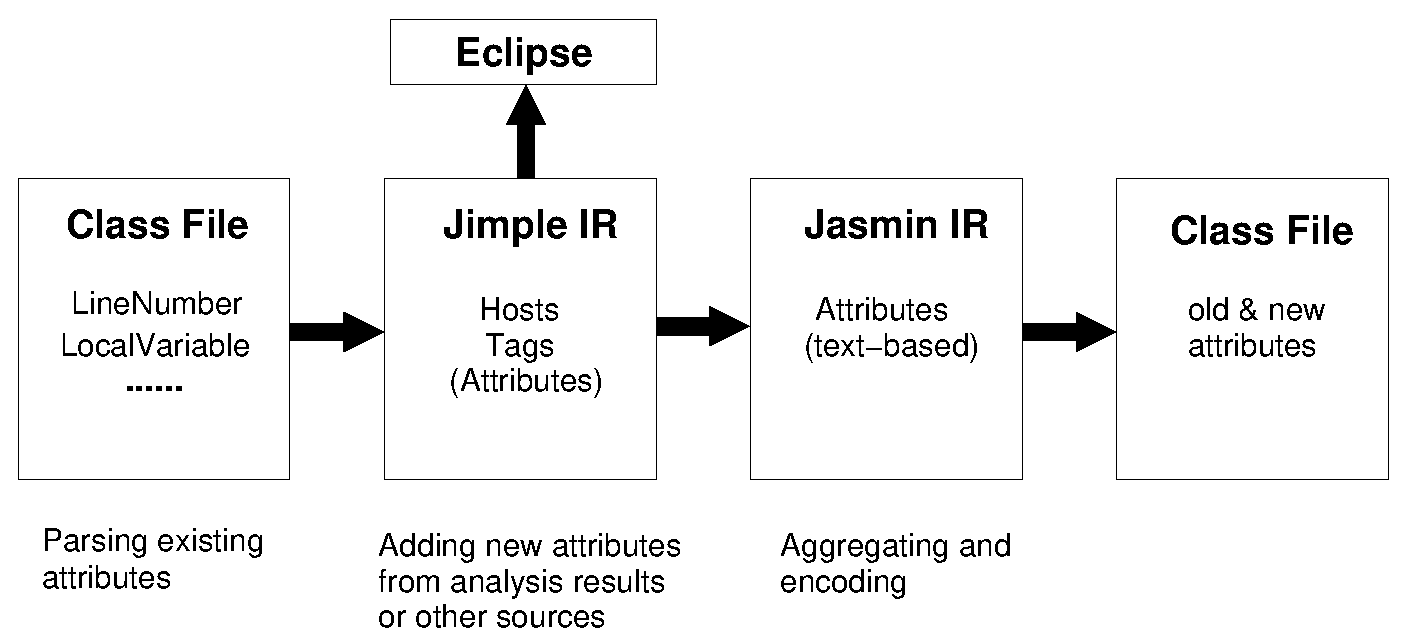
\epsfig{file=soot-attribute.eps,width=4.3in}
\begin{itemize}
\item Soot parses several standard attributes 
\item New attributes can be created and attached 
\item Users can design their own attribute format
\end{itemize}
\end{slide}

%% a picture shows mapping between soot internal objects to class file structures
\begin{slide}{Tags in Soot Internals}
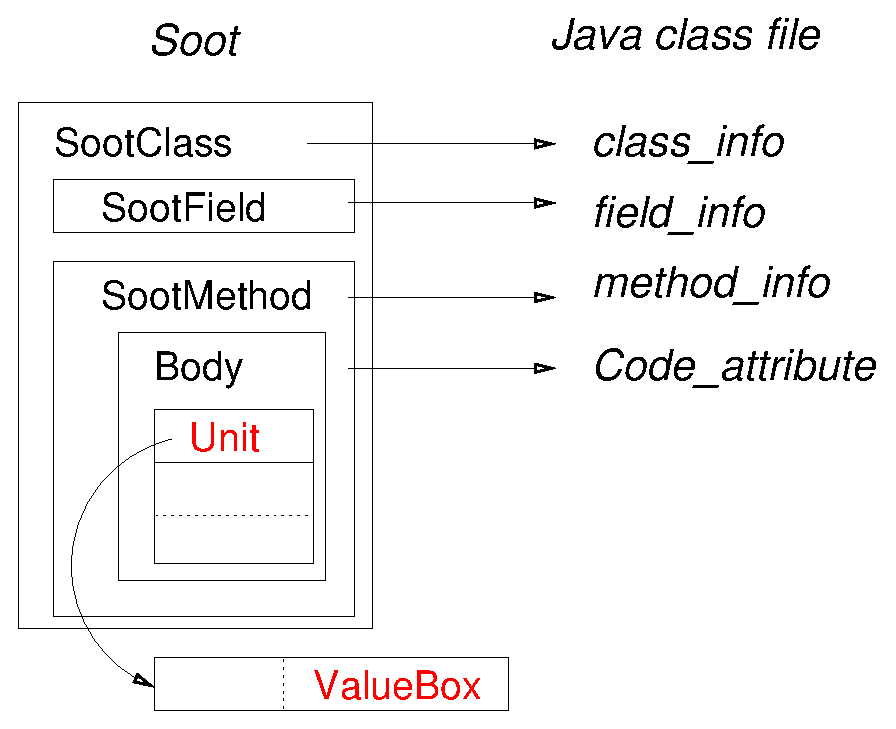
\epsfig{file=attr-map.eps,width=3.5in}
\end{slide}

\begin{slide}{Hosts}
{\red Host}s are objects that can hold {\red Tag}s:
{\small
\begin{verbatim}
package soot.tagkit;
public interface Host {
  public void addTag (Tag t); 
  public Tag getTag (String aName); 
  public List getTags ();
  public void removeTag (String name); 
  public boolean hasTag (String aName); 
}   
\end{verbatim}
}
Implementations:\\
{\small SootClass, SootField, SootMethod, Body, Unit, ValueBox}
\end{slide}

\begin{slide}{Tags}
{\red Tag}s are objects that can be attached to {\red Host}s:
\small{
\begin{verbatim}
package soot.tagkit;
public interface Tag {
  public String getName ();  
  public byte[] getValue () 
    throws AttributeValueException; 
  public String toString();
}
\end{verbatim}
}
\begin{itemize}
\item {\red Attribute} attached to class file structures (class, field, method)
\item Generic tags attached to {\em Unit}s or {\em ValueBox}es
\end{itemize}
\end{slide}

\begin{slide}{Tag Hierarchy}
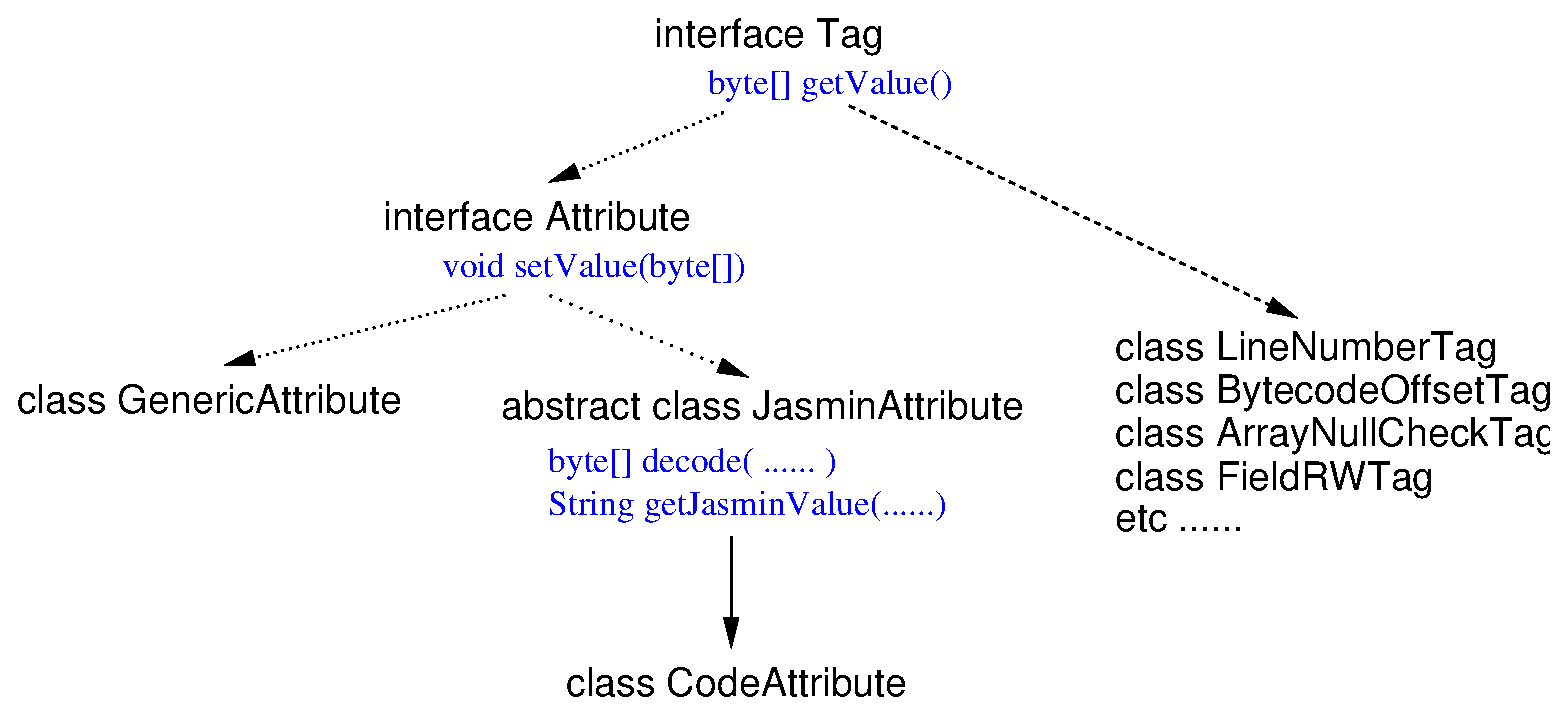
\epsfig{file=tag-hierarchy.eps, width=4.2in}
\end{slide}

%% how does soot produce tags and attributes in class file
\begin{slide}{Special case: attributes of Code\_attribute}
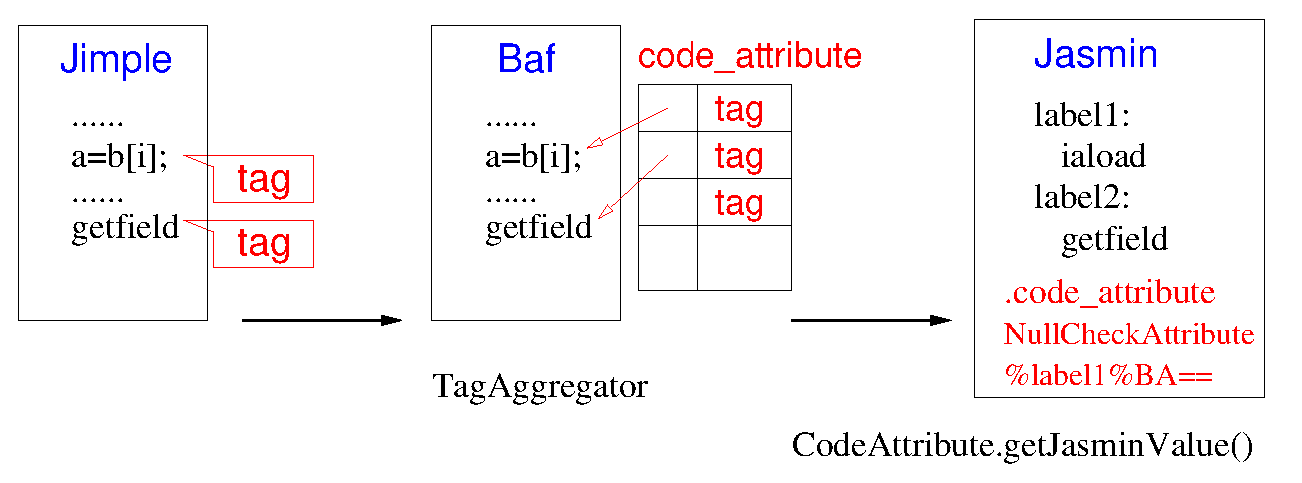
\epsfig{file=attr-flow.eps, width=4.2in}

\begin{itemize}
\item {\red TagAggregator} aggregates tags of Units/ValueBoxes to {\red CodeAttribute}
\item CodeAttribute is a table of (pc, value) pairs in class file
\end{itemize}
\end{slide}

\begin{slide}{Choosing an Aggregator}
\begin{itemize}
\item One Jimple statement may translate to multiple bytecode instructions\\
\ \\
\begin{minipage}[t]{45mm}
Jimple
\begin{alltt}
x = y.f
\end{alltt}
\end{minipage}
\begin{minipage}[t]{45mm}
Bytecode
\begin{alltt}
load y
getfield f
store x
\end{alltt}
\end{minipage}
\item Which instruction(s) should get the tags?
\end{itemize}
\end{slide}

\begin{slide}{Choosing an Aggregator}
\begin{description}
\item [ImportantTagAggregator]\ \\
attaches tag to the {\bf ``most important''} instruction
(field reference, array reference, method invocation)
\begin{itemize}
\item Used for array bounds check, null pointer check, side-effect attributes
\end{itemize}
\item [FirstTagAggregator]\ \\
attaches tag to the {\bf first} instruction
\begin{itemize}
\item Used for line number table attribute
\end{itemize}
\item Easy to make your own \ldots
\end{description}
\end{slide}


\begin{slide}{TagAggregator}
{\small
\begin{verbatim}
public abstract class TagAggregator 
  extends BodyTransformer {
  ......
  abstract boolean wantTag(Tag t);
  abstract void considerTag(Tag t, Unit u);
  abstract String aggregatedName();
  void internalTransform(Body b, ... ) { 
    ...... 
  }
}
\end{verbatim}
}
\end{slide}

\begin{slide}{ImportantTagAggregator}
\vspace*{-6mm}
\begin{verbatim}
abstract class ImportantTagAggregator 
extends TagAggregator {    
    /** Decide whether this tag
     *  should be aggregated by
     *  this aggregator. */
    public abstract boolean
                    wantTag( Tag t );

    /** Return name of the resulting
     *  aggregated tag. */
    public abstract String 
                    aggregatedName();
}
\end{verbatim}
\end{slide}

\begin{slide}{Howto for creating new attributes}
\begin{itemize}
\item Create a new Tag class, decide which structure is the host
\item If the tag is for Units, write a tag aggregator by extending {\em TagAggregator} or one of its subclasses
\item Parse attributes in bytecode consumer
\end{itemize}
\end{slide}

\begin{slide}{Example: nullness attribute}
Step 1: create NullCheckTag
{\scriptsize
\begin{verbatim}
class NullCheckTag {
  public String getName() { return "NullCheckTag"; }
  private byte value = 0;
  public byte[] getValue() {
    byte[] bv = new byte[1];
    bv[0] = value;
    return bv;
  }
  public void toString() {
    return ((value==0)?"[not null]":"[unknown]");
  }
}
\end{verbatim}
}
\end{slide}

\begin{slide}{Example: nullness attribute}
Step 2: attach tags to units after analysis \\
\footnotesize{
\begin{verbatim}
boolean needCheck;
s.addTag(new NullCheckTag(needCheck));
\end{verbatim}
}
\end{slide}

\begin{slide}{Example: nullness attribute}
Step 3: create a NullTagAggregator
{\scriptsize\verb$p.add(new Transform("tag.null",$
   \verb$         NullTagAggregator.v())); $}
\ \\
\ \\
{\scriptsize
\begin{verbatim}
class NullTagAggregator
        extends ImportantTagAggregator {

    public boolean wantTag(Tag t) {
        return (t instanceof NullCheckTag);
    }
    public String aggregatedName() {
        return "NullCheckAttribute"; 
    }
}
\end{verbatim}
}
\end{slide}

\begin{slide}{Code attribute format}
Attributes of Code\_attribute extends {\em JasminAttribute}
which generates textual representation of (label, value)
pairs:\\
\footnotesize{\verb$ String getJasminValue(Map instToLabel); $} \\
e.g. "NullCheckAttribute":
\footnotesize{
\begin{verbatim}
null_check_attribute {
  u2 attribute_name_index;
  u4 attribute_length;
  {   u2 pc;
      u1 data;
  } [attribute_length/3];
}
\end{verbatim}
}
\end{slide}
